\documentclass[11pt,a4paper]{article}

\usepackage[margin=2.5cm]{geometry}
\usepackage{graphicx}
\usepackage{listings}
\usepackage{xcolor}
\usepackage{hyperref}
\usepackage[spanish]{babel}

% --- Estilo de código C# ---
\lstdefinestyle{csharp}{
    language=[Sharp]C,
    basicstyle=\ttfamily\small,
    keywordstyle=\color{blue},
    commentstyle=\color{gray},
    stringstyle=\color{orange},
    numbers=left,
    numberstyle=\tiny,
    frame=single,
    breaklines=true,
    showstringspaces=false
}

% --- Estilo de código JSON/HTTP ---
\lstdefinestyle{json}{
    basicstyle=\ttfamily\small,
    frame=single,
    breaklines=true,
    showstringspaces=false
}

\title{Depreciacion App \\ \large Informe Técnico de Arquitectura}
\author{[Nombre integrante 1] \\ [Nombre integrante 2]}
\date{\today}

\begin{document}

\maketitle
\tableofcontents
\newpage

\section{Introducción}
% TODO (agente informe): qué hace el sistema, alcance, tecnologías y por qué cada una.

\section{Justificación de la arquitectura de microservicios}

El sistema se divide en dos servicios .NET 8 independientes que se comunican
por HTTP, sin API Gateway ni contenedores. Cada uno cumple las cuatro
características que definen un microservicio, con evidencia concreta en el
código del repositorio.

\subsection{Business Function}

\textbf{Definición}: cada microservicio resuelve una única responsabilidad de
negocio, no un conjunto de funciones técnicas mezcladas.

En este proyecto la división es explícita: \texttt{AuthService} se ocupa
únicamente de la autenticación (login y firma de JWT), y
\texttt{AssetsService} de la gestión y el cálculo de activos. Cada servicio
expone su propio controlador con rutas REST dedicadas:

\begin{lstlisting}[style=csharp, caption={AuthService.Api/Controllers/AuthController.cs (fragmento)}]
[ApiController]
[Route("api/auth")]
public class AuthController : ControllerBase
{
    [HttpPost("login")]
    public async Task<IActionResult> Login([FromBody] LoginRequest request)
    {
        var response = await _login.EjecutarAsync(request);
        ...
    }
}
\end{lstlisting}

\begin{lstlisting}[style=csharp, caption={AssetsService.Api/Controllers/ActivosController.cs (fragmento)}]
[Authorize]
[ApiController]
[Route("api/activos")]
public class ActivosController : ControllerBase
{
    [HttpPost]
    public async Task<IActionResult> Crear([FromBody] ActivoRequest request) ...

    [HttpGet("{id}/depreciacion")]
    public async Task<IActionResult> Depreciacion(int id) ...
}
\end{lstlisting}

\textbf{Por qué aplica}: \texttt{AuthController} solo conoce credenciales y
tokens; \texttt{ActivosController} solo conoce activos y depreciación. Ningún
controlador mezcla ambas responsabilidades, y cada servicio puede evolucionar
su lógica sin afectar al otro.

\subsection{API Communication}

\textbf{Definición}: los microservicios se comunican exclusivamente por API
REST sobre HTTP; no comparten memoria, objetos ni proceso.

Ambos servicios exponen endpoints REST y el frontend los consume por HTTP. El
archivo \texttt{frontend/src/api.js} define las dos URLs base y usa
\texttt{fetch} para cada llamada:

\begin{lstlisting}[style=json, caption={frontend/src/api.js (fragmento)}]
const AUTH_URL = 'http://localhost:5001'
const ASSETS_URL = 'http://localhost:5002'

export async function login(username, password) {
  return request(`${AUTH_URL}/api/auth/login`, { ... })
}

export async function listarActivos() {
  return request(`${ASSETS_URL}/api/activos`, { headers: authHeaders() })
}
\end{lstlisting}

\textbf{Por qué aplica}: cada petición viaja como JSON sobre HTTP y el
servidor responde con JSON; no hay llamadas directas entre procesos ni
variables compartidas entre servicios.

\subsection{Independent Operation}

\textbf{Definición}: cada microservicio corre como un proceso independiente,
con su propio puerto, su propia configuración y su propia base de datos; se
puede detener uno sin tumbar al otro.

Cada servicio se levanta con su propio \texttt{dotnet run} en un puerto
distinto (\texttt{launchSettings.json}) y apunta a su propia base de datos
(\texttt{appsettings.json}):

\begin{lstlisting}[style=json, caption={AuthService.Api/Properties/launchSettings.json (fragmento)}]
"profiles": {
    "http": {
      "applicationUrl": "http://localhost:5001",
      ...
    }
}
\end{lstlisting}

\begin{lstlisting}[style=json, caption={AssetsService.Api/Properties/launchSettings.json (fragmento)}]
"profiles": {
    "http": {
      "applicationUrl": "http://localhost:5002",
      ...
    }
}
\end{lstlisting}

\begin{lstlisting}[style=json, caption={appsettings.json de cada servicio (fragmentos)}]
// AuthService.Api/appsettings.json
"ConnectionStrings": {
    "AuthDB": "Server=localhost;Database=AuthDB;User Id=auth_user;..."
}

// AssetsService.Api/appsettings.json
"ConnectionStrings": {
    "AssetsDB": "Server=localhost;Database=AssetsDB;User Id=assets_user;..."
}
\end{lstlisting}

\textbf{Por qué aplica}: cada servicio tiene su propio puerto (5001 y 5002) y
su propia base de datos (AuthDB y AssetsDB) con usuarios de SQL Server
distintos (\texttt{auth\_user} y \texttt{assets\_user}); detener
\texttt{AuthService} no impide que \texttt{AssetsService} siga respondiendo.

\subsection{Request Handling}

\textbf{Definición}: el enrutamiento de cada petición hacia el microservicio
correcto es una decisión explícita; en este caso la toma el cliente (no hay
API Gateway).

El frontend decide a qué servicio llamar según la operación, en
\texttt{frontend/src/api.js}: login siempre va a \texttt{AUTH\_URL} (5001) y
las operaciones de activos/depreciación a \texttt{ASSETS\_URL} (5002):

\begin{lstlisting}[style=json, caption={frontend/src/api.js (fragmento)}]
// ---------- AuthService (puerto 5001) ----------
export async function login(username, password) {
  return request(`${AUTH_URL}/api/auth/login`, { ... })
}

// ---------- AssetsService (puerto 5002) ----------
export async function obtenerDepreciacion(id) {
  return request(`${ASSETS_URL}/api/activos/${id}/depreciacion`, { ... })
}
\end{lstlisting}

\textbf{Por qué aplica}: no existe un gateway central; el enrutamiento es
explícito en el código del cliente, lo que simplifica la infraestructura
(acorde con la decisión de no usar contenedores) manteniendo el desacople
entre servicios.

% Diagrama generado desde diagramas/contenedores.mmd -> diagramas/contenedores.png
\begin{figure}[h]
    \centering
    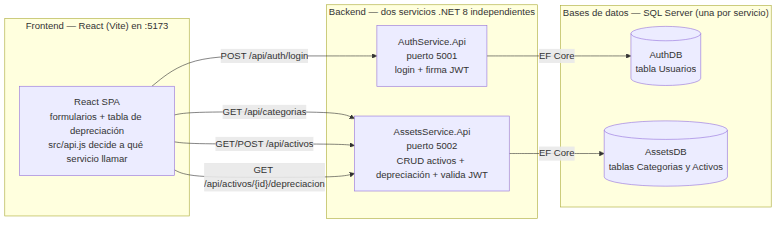
\includegraphics[width=0.9\textwidth]{diagramas/contenedores.png}
    \caption{Diagrama de contenedores del sistema}
    \label{fig:contenedores}
\end{figure}

\section{Justificación de Onion Architecture}

\textbf{Por qué Onion y no una arquitectura en capas simple}: en una
arquitectura en capas tradicional (Controllers $\rightarrow$ Services
$\rightarrow$ Repositories $\rightarrow$ DbContext), la capa de persistencia
es la más interna y todo depende de ella: si se cambia el motor de base de
datos, se reescribe el resto. Onion Architecture invierte esa dependencia: el
\textbf{Domain} (reglas de negocio) queda en el centro sin depender de nada,
y la persistencia pasa a la periferia, dependiendo de las interfaces que el
centro define.

La regla de dependencia se cumple a nivel de compilador porque cada capa es
un proyecto .NET separado:

\begin{itemize}
    \item \texttt{Domain} no referencia a nadie.
    \item \texttt{Application} referencia solo a \texttt{Domain}.
    \item \texttt{Infrastructure} referencia a \texttt{Application} y \texttt{Domain}.
    \item \texttt{Api} referencia a los tres (es quien hace el cableado final).
\end{itemize}

La verificación con \texttt{dotnet list reference} confirma la regla en el
proyecto más interno:

\begin{lstlisting}[style=json, caption={Verificación de la regla de dependencia}]
$ dotnet list AssetsService.Domain/AssetsService.Domain.csproj reference
There are no Project to Project references in project
AssetsService.Domain/AssetsService.Domain.csproj.
\end{lstlisting}

El archivo \texttt{AssetsService.Domain.csproj} lo confirma: no contiene
ningún \texttt{ProjectReference} ni paquete de persistencia:

\begin{lstlisting}[style=json, caption={AssetsService.Domain/AssetsService.Domain.csproj}]
<Project Sdk="Microsoft.NET.Sdk">
  <PropertyGroup>
    <TargetFramework>net8.0</TargetFramework>
    <ImplicitUsings>enable</ImplicitUsings>
    <Nullable>enable</Nullable>
  </PropertyGroup>
</Project>
\end{lstlisting}

El beneficio concreto: \texttt{Domain} y \texttt{Application} nunca importan
\texttt{Microsoft.EntityFrameworkCore}; la persistencia es un detalle
intercambiable que vive en \texttt{Infrastructure}.

% Diagrama generado desde diagramas/onion.mmd -> diagramas/onion.png
\begin{figure}[h]
    \centering
    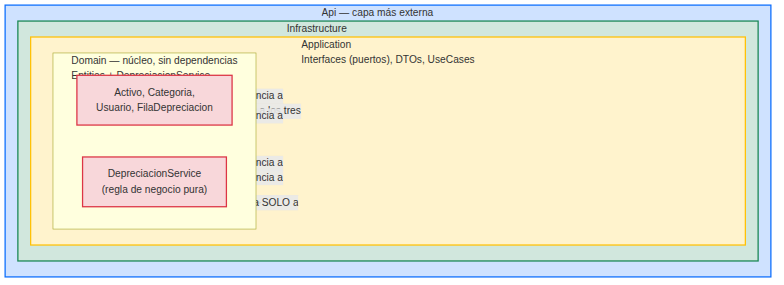
\includegraphics[width=0.7\textwidth]{diagramas/onion.png}
    \caption{Anillos de Onion Architecture aplicados al proyecto}
    \label{fig:onion}
\end{figure}

\section{Contraste de conceptos de Clean/Onion Architecture contra el código real}

\subsection{Entidades de dominio}
% TODO: definición + \begin{lstlisting}[style=csharp] ... \end{lstlisting} + por qué aplica

\subsection{Reglas de negocio en el dominio}
% TODO

\subsection{Casos de uso (capa de Aplicación)}
% TODO

\subsection{Inversión de dependencias}
% TODO: interfaz en Application + implementación en Infrastructure

\subsection{DTOs como contrato de frontera}
% TODO

\subsection{Inyección de dependencias}
% TODO: fragmento de Program.cs

\section{Modelo de datos}
% TODO: por qué database-per-service

% Diagrama generado desde diagramas/modelo-datos.mmd -> diagramas/modelo-datos.png
\begin{figure}[h]
    \centering
    % 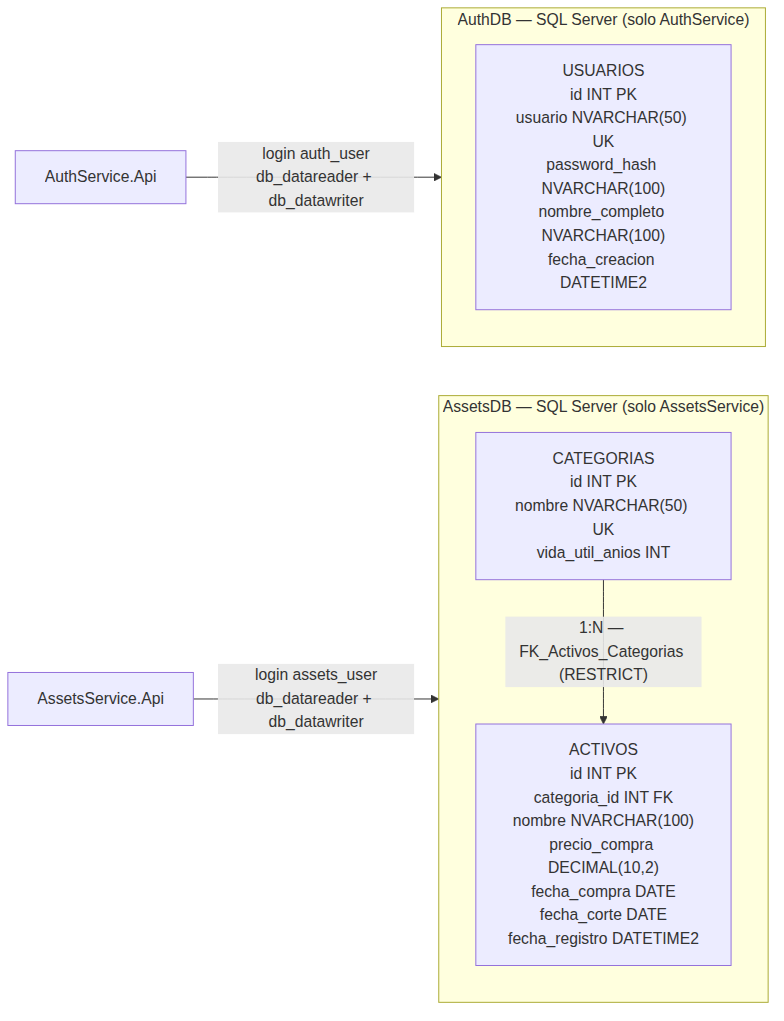
\includegraphics[width=0.8\textwidth]{diagramas/modelo-datos.png}
    \caption{Modelo entidad-relación}
    \label{fig:er}
\end{figure}

\section{Flujos principales}

\subsection{Autenticación}
% Diagrama generado desde diagramas/secuencia-login.mmd -> diagramas/secuencia-login.png
\begin{figure}[h]
    \centering
    % 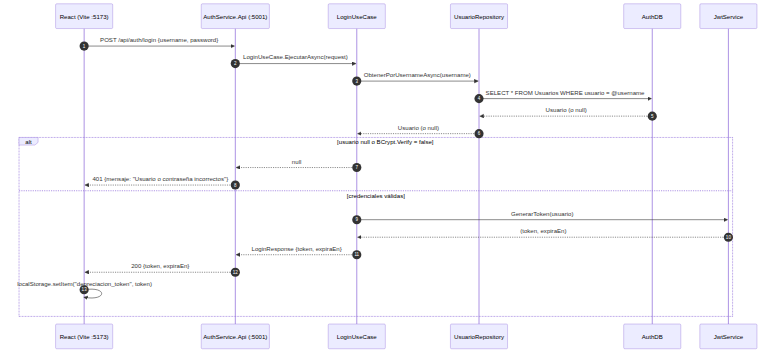
\includegraphics[width=0.9\textwidth]{diagramas/secuencia-login.png}
    \caption{Secuencia de login}
\end{figure}

\subsection{Creación y consulta de depreciación}
% Diagrama generado desde diagramas/secuencia-depreciacion.mmd -> diagramas/secuencia-depreciacion.png
\begin{figure}[h]
    \centering
    % 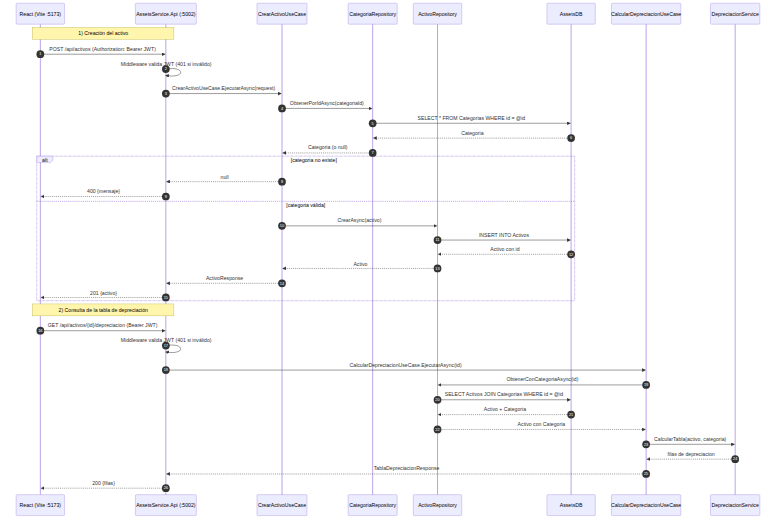
\includegraphics[width=0.9\textwidth]{diagramas/secuencia-depreciacion.png}
    \caption{Secuencia de creación de activo y cálculo de depreciación}
\end{figure}

\section{Corrección de la lógica de depreciación}
% TODO: algoritmo años completos + resto parcial, ejemplo numérico oficial, código real.

\section{Pruebas}
% TODO: casos probados y por qué, con nombres reales de los métodos de test.

\section{Flujo de trabajo (Git)}
% TODO: resumen del Git Flow simplificado.

\section{Conclusiones}
% TODO: decisiones de alcance tomadas conscientemente.

\end{document}
